%\documentclass[a4paper]{fhnwreport} %Legt grundlegende Formatierungen wie Schriftarten, Ort Seitenzahlen etc. fest.
%
%\graphicspath{{./graphics/}}%Change according to graphics folder!
%
%\begin{document}

\section{Hardware}

Der Sensorprint wird über das Solarpanel gespiesen. Es ist deshalb darauf zu achten, das die Leistung nicht mehr als 100mW beträgt.

Die Kommunikation über die Powerline (PLC) wird mittels eines Powerline Transceivers/Receivers realisiert.
\begin{figure}[h]
\centering
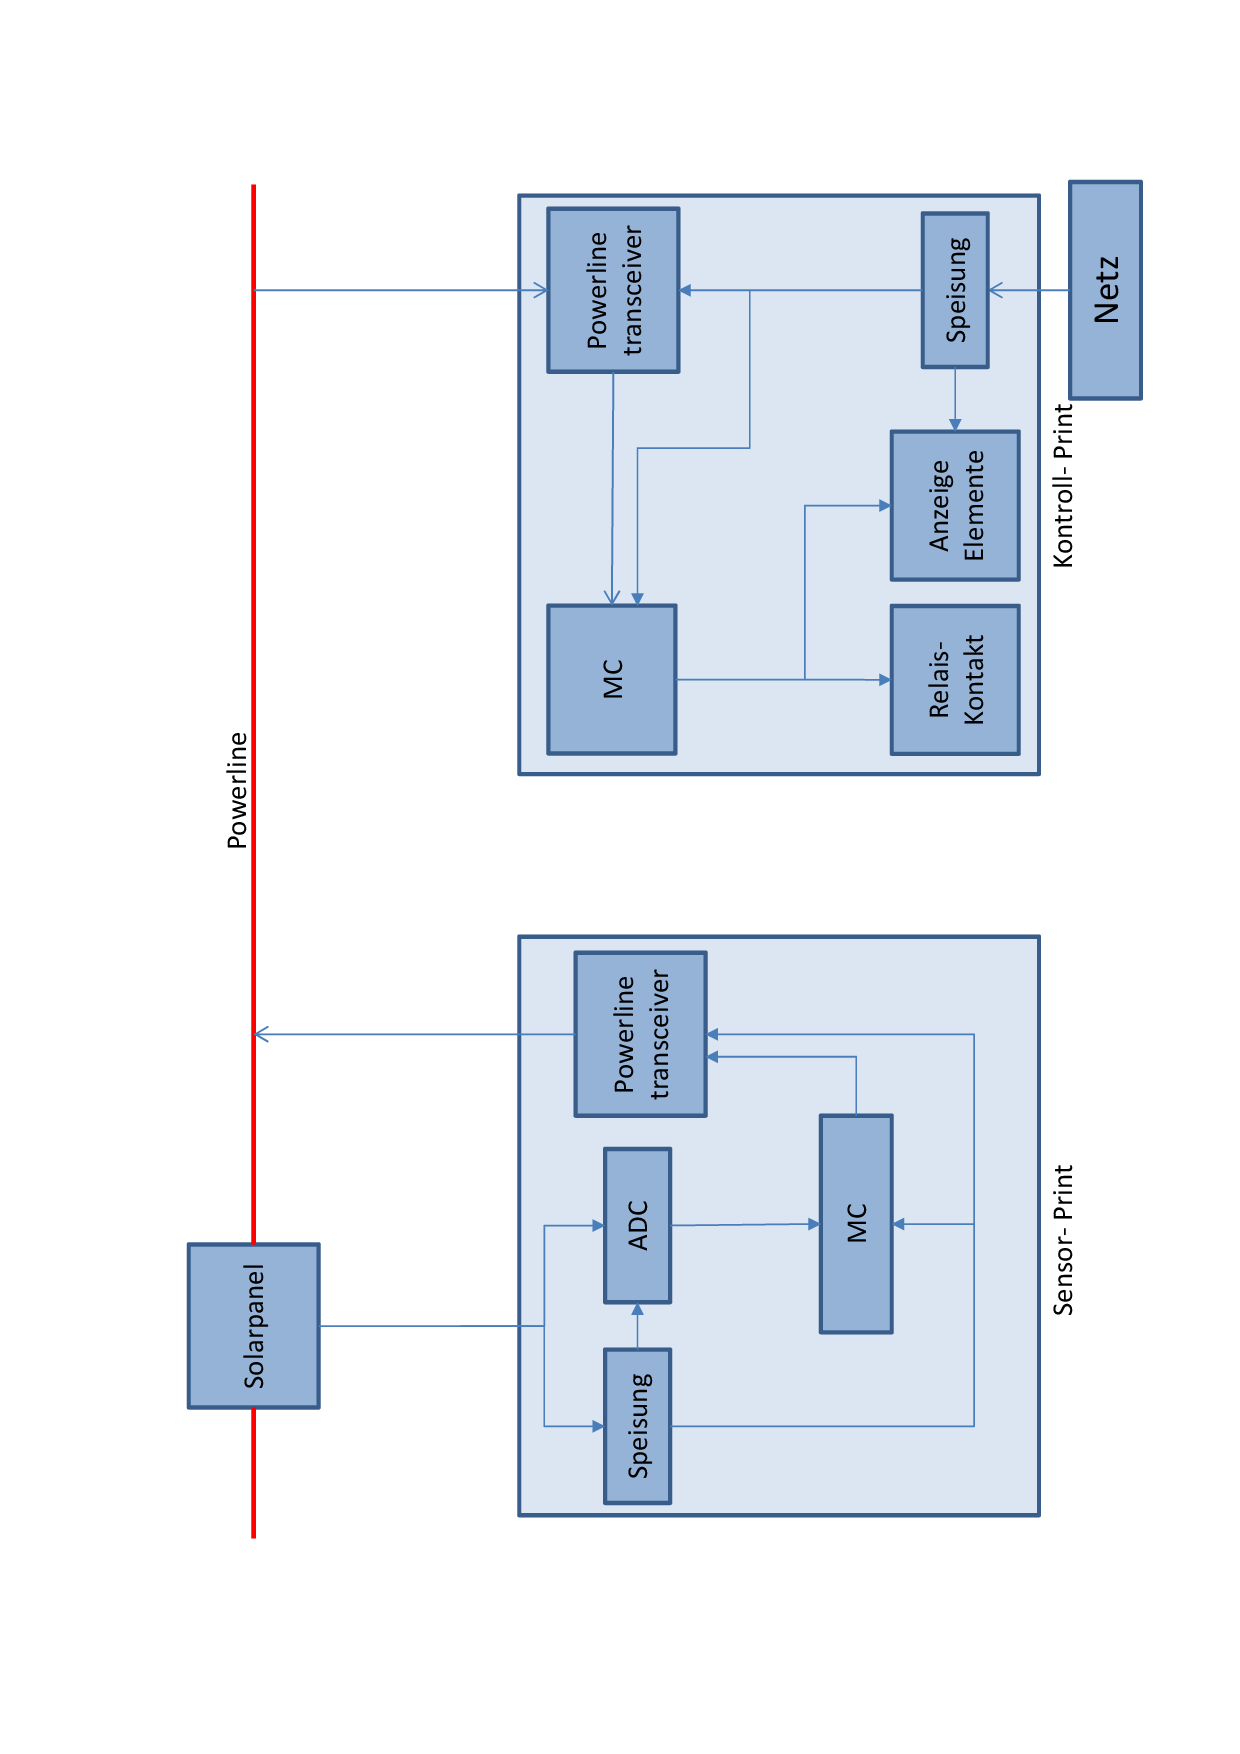
\includegraphics[angle = -90, width=1.0\textwidth]{Hardware_Konzept.png}%
\caption{Hardwarekonzept}
\label{fig::Hardwarekonzept}%
\end{figure}

\subsection{Sensorplatine}

\subsection{Kontrollplatine}
%\end{document}
